
\section{Appendix-A: KDD-NSL Dataset}
\label{appendix-1}
\begin{figure*}[h!]
     \centering
     \begin{subfigure}{0.47\textwidth}
         \centering
         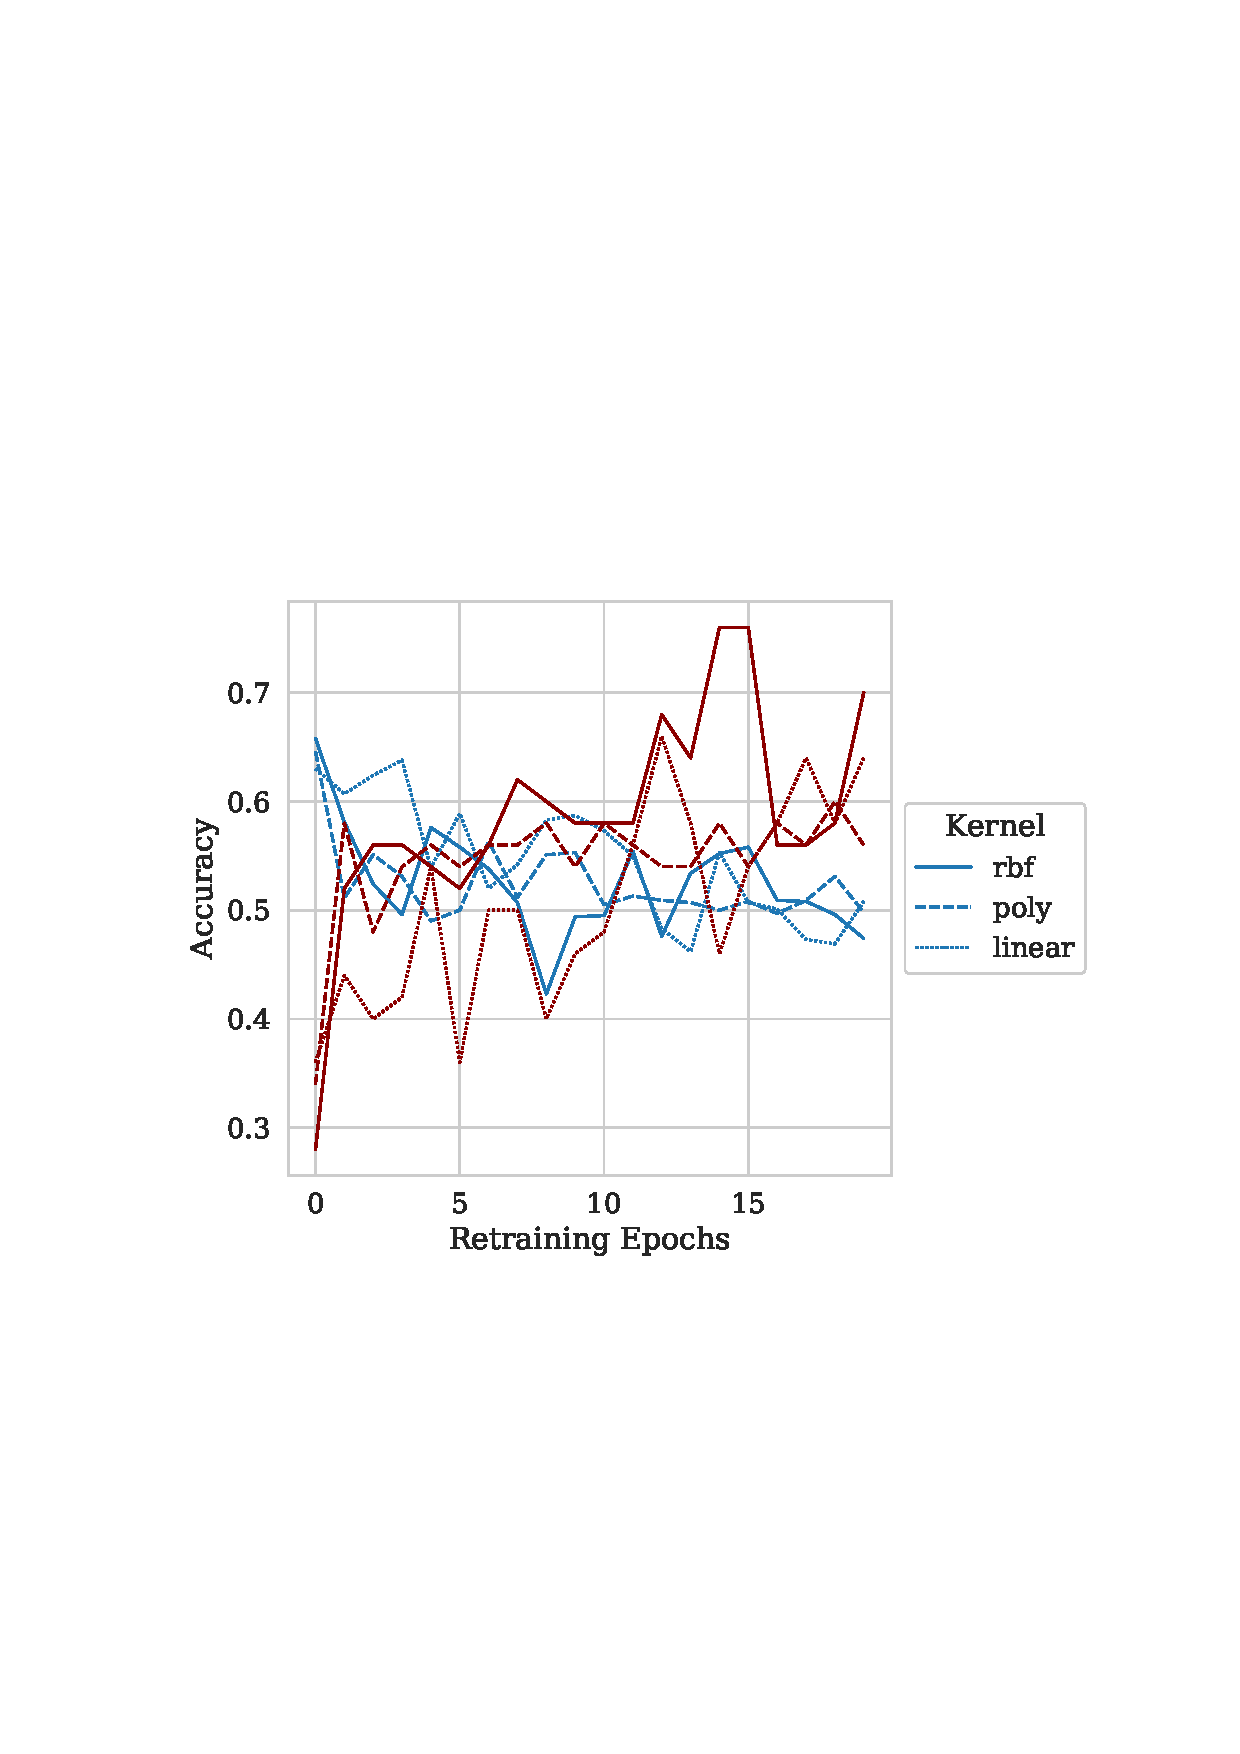
\includegraphics[width=\textwidth]{./kdd-nsl/retrain_accuracy.pdf}
     \end{subfigure}
     \hfill
     \begin{subfigure}{0.47\textwidth}
         \centering
         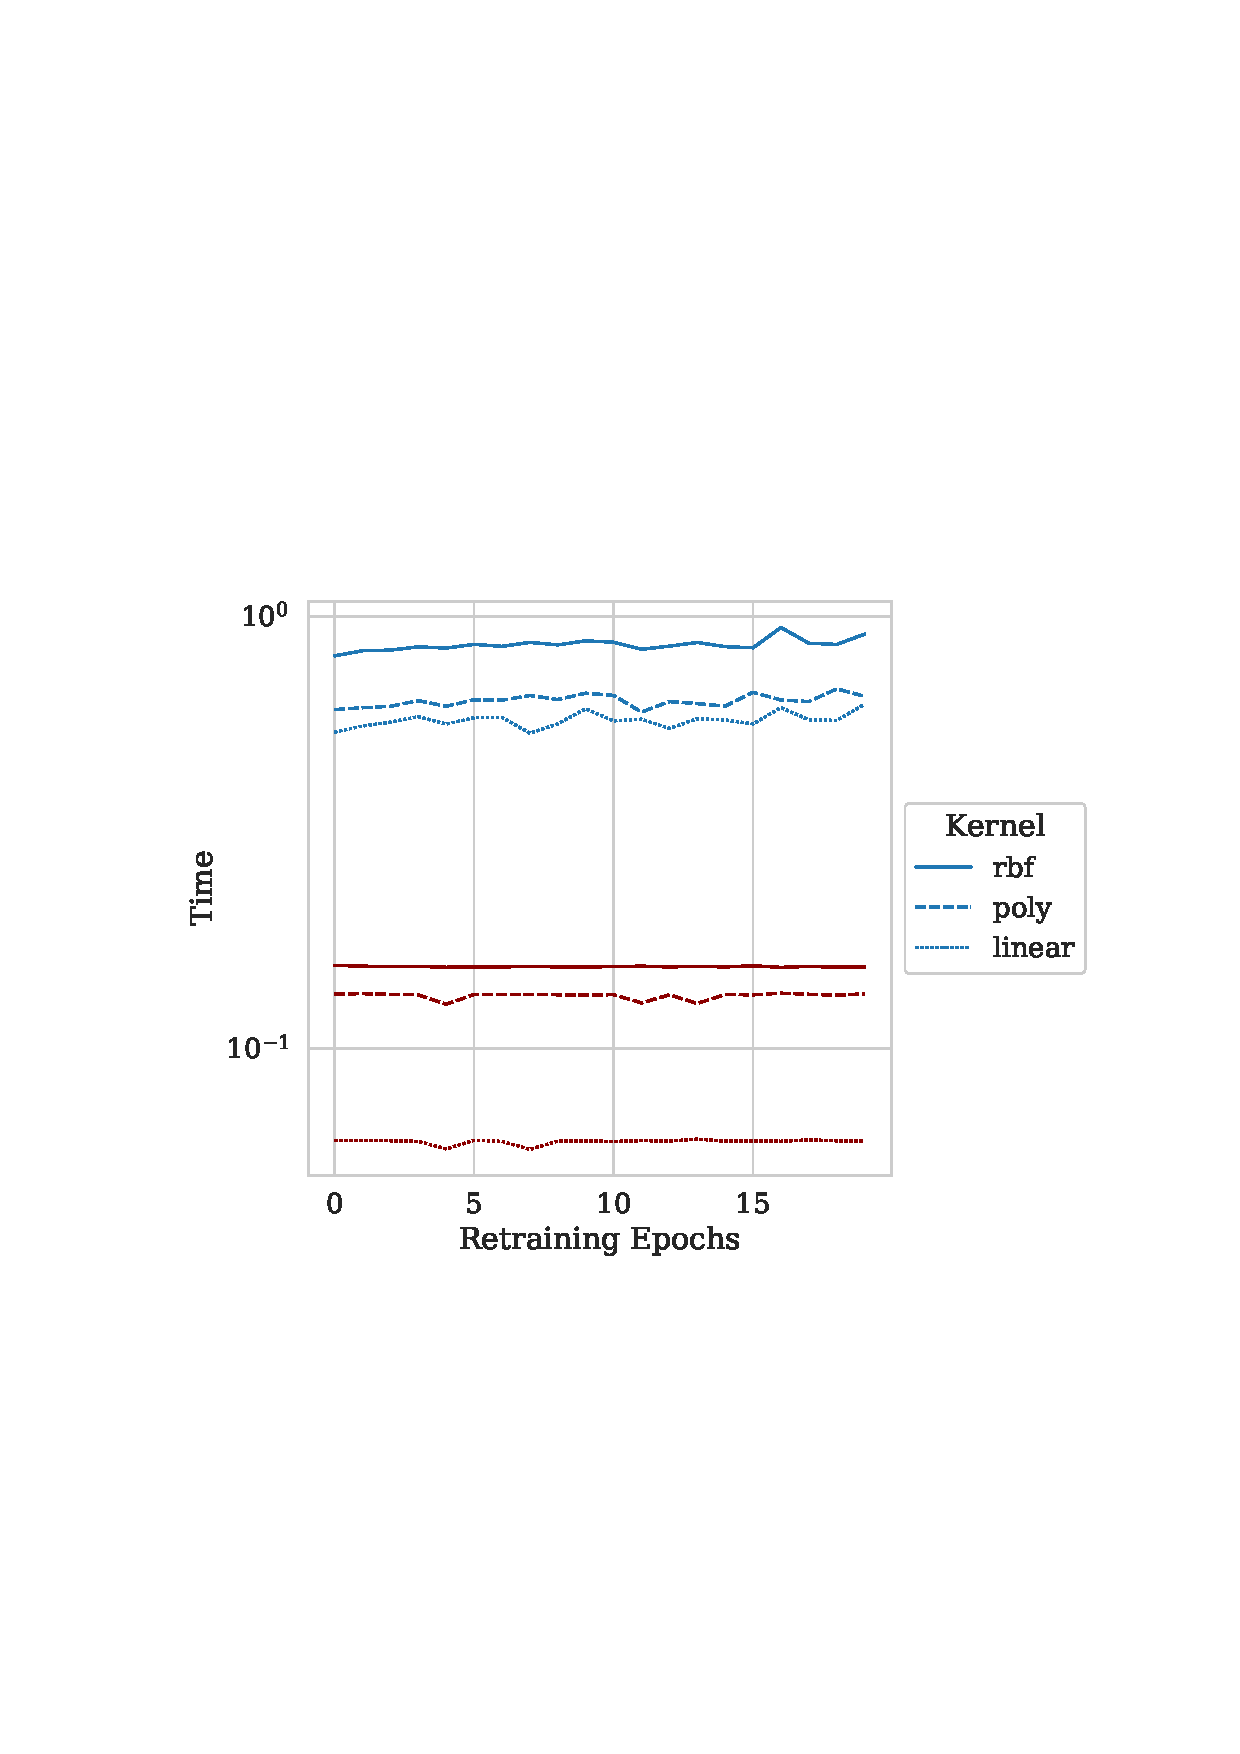
\includegraphics[width=\textwidth]{./kdd-nsl/retrain_time.pdf}
     \end{subfigure}
     \hfill
     \begin{subfigure}{0.47\textwidth}
         \centering
         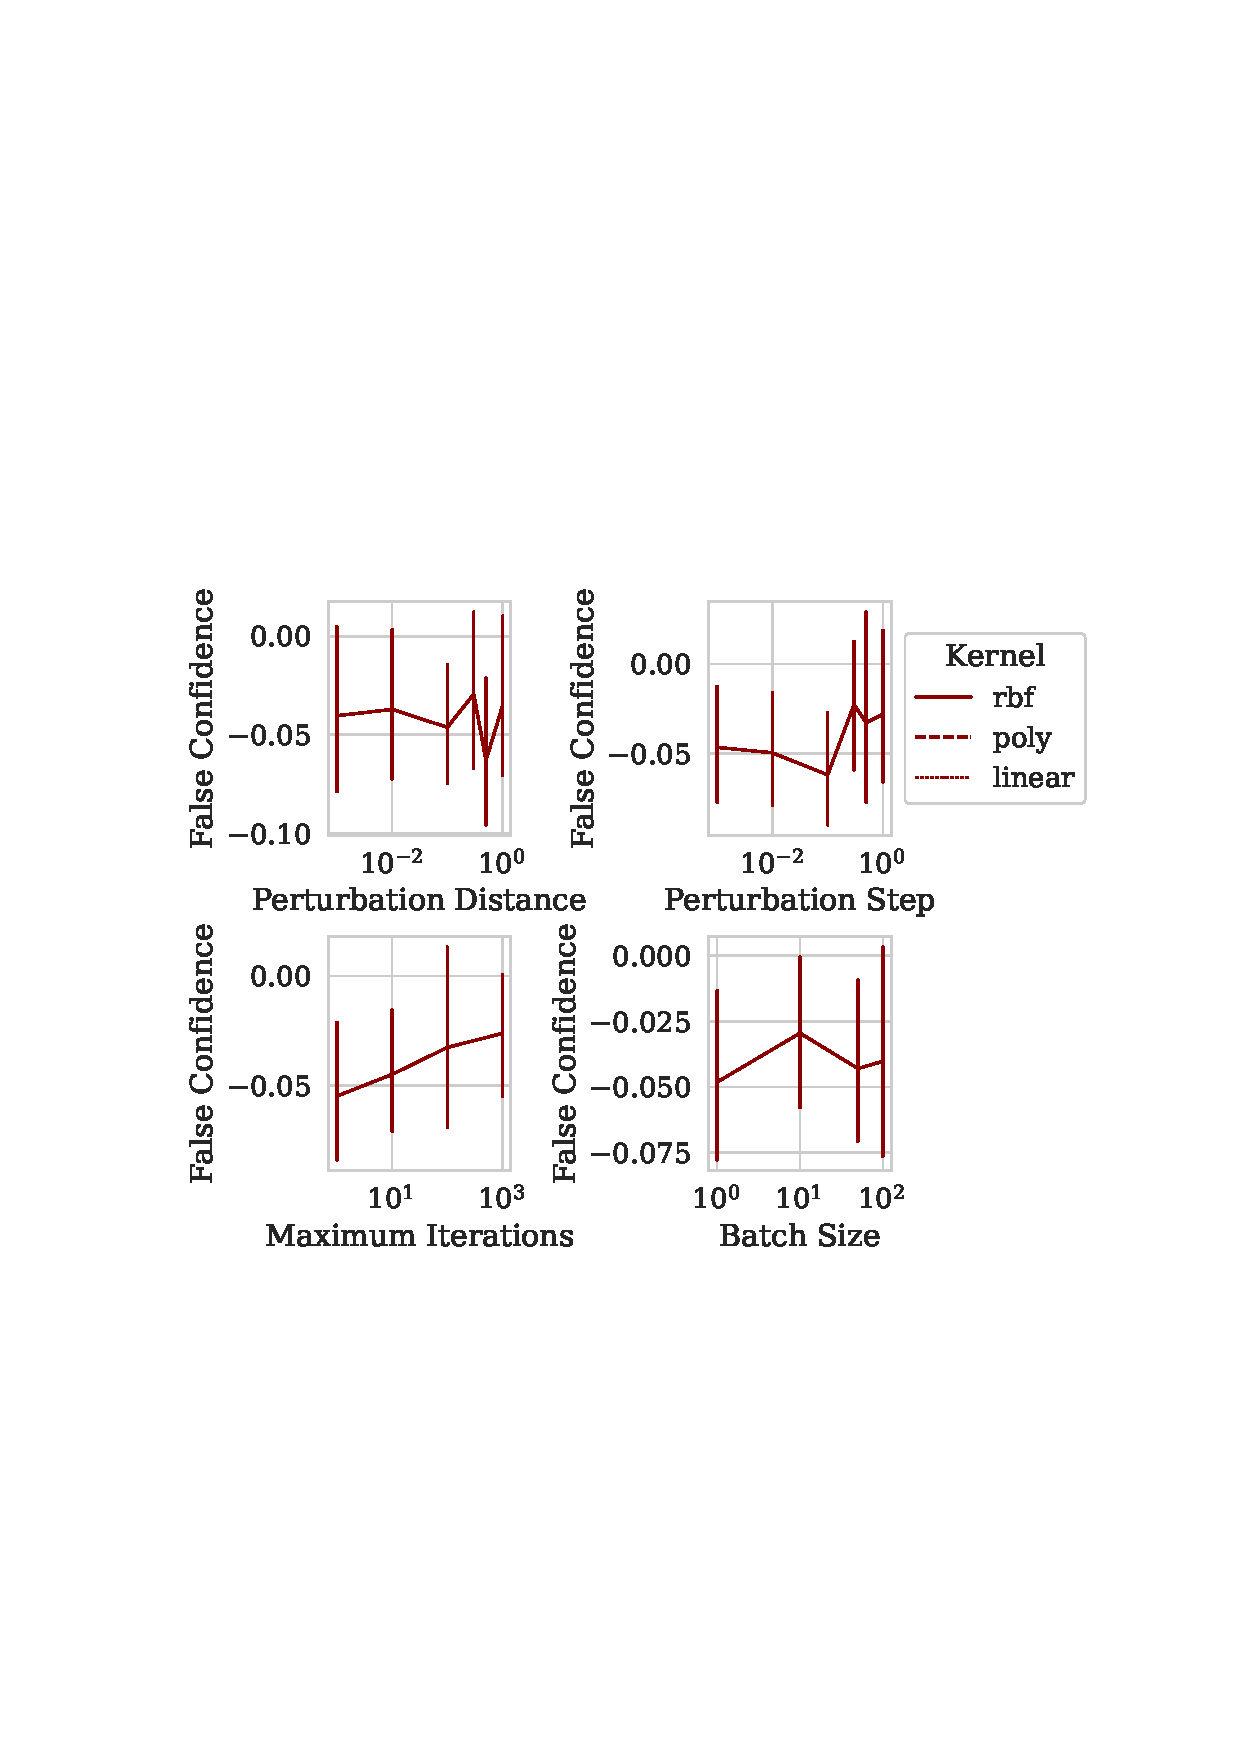
\includegraphics[width=\textwidth]{./kdd-nsl/confidence_vs_attack_parameters.pdf}
     \end{subfigure}
     \hfill
     \begin{subfigure}{0.47\textwidth}
         \centering
         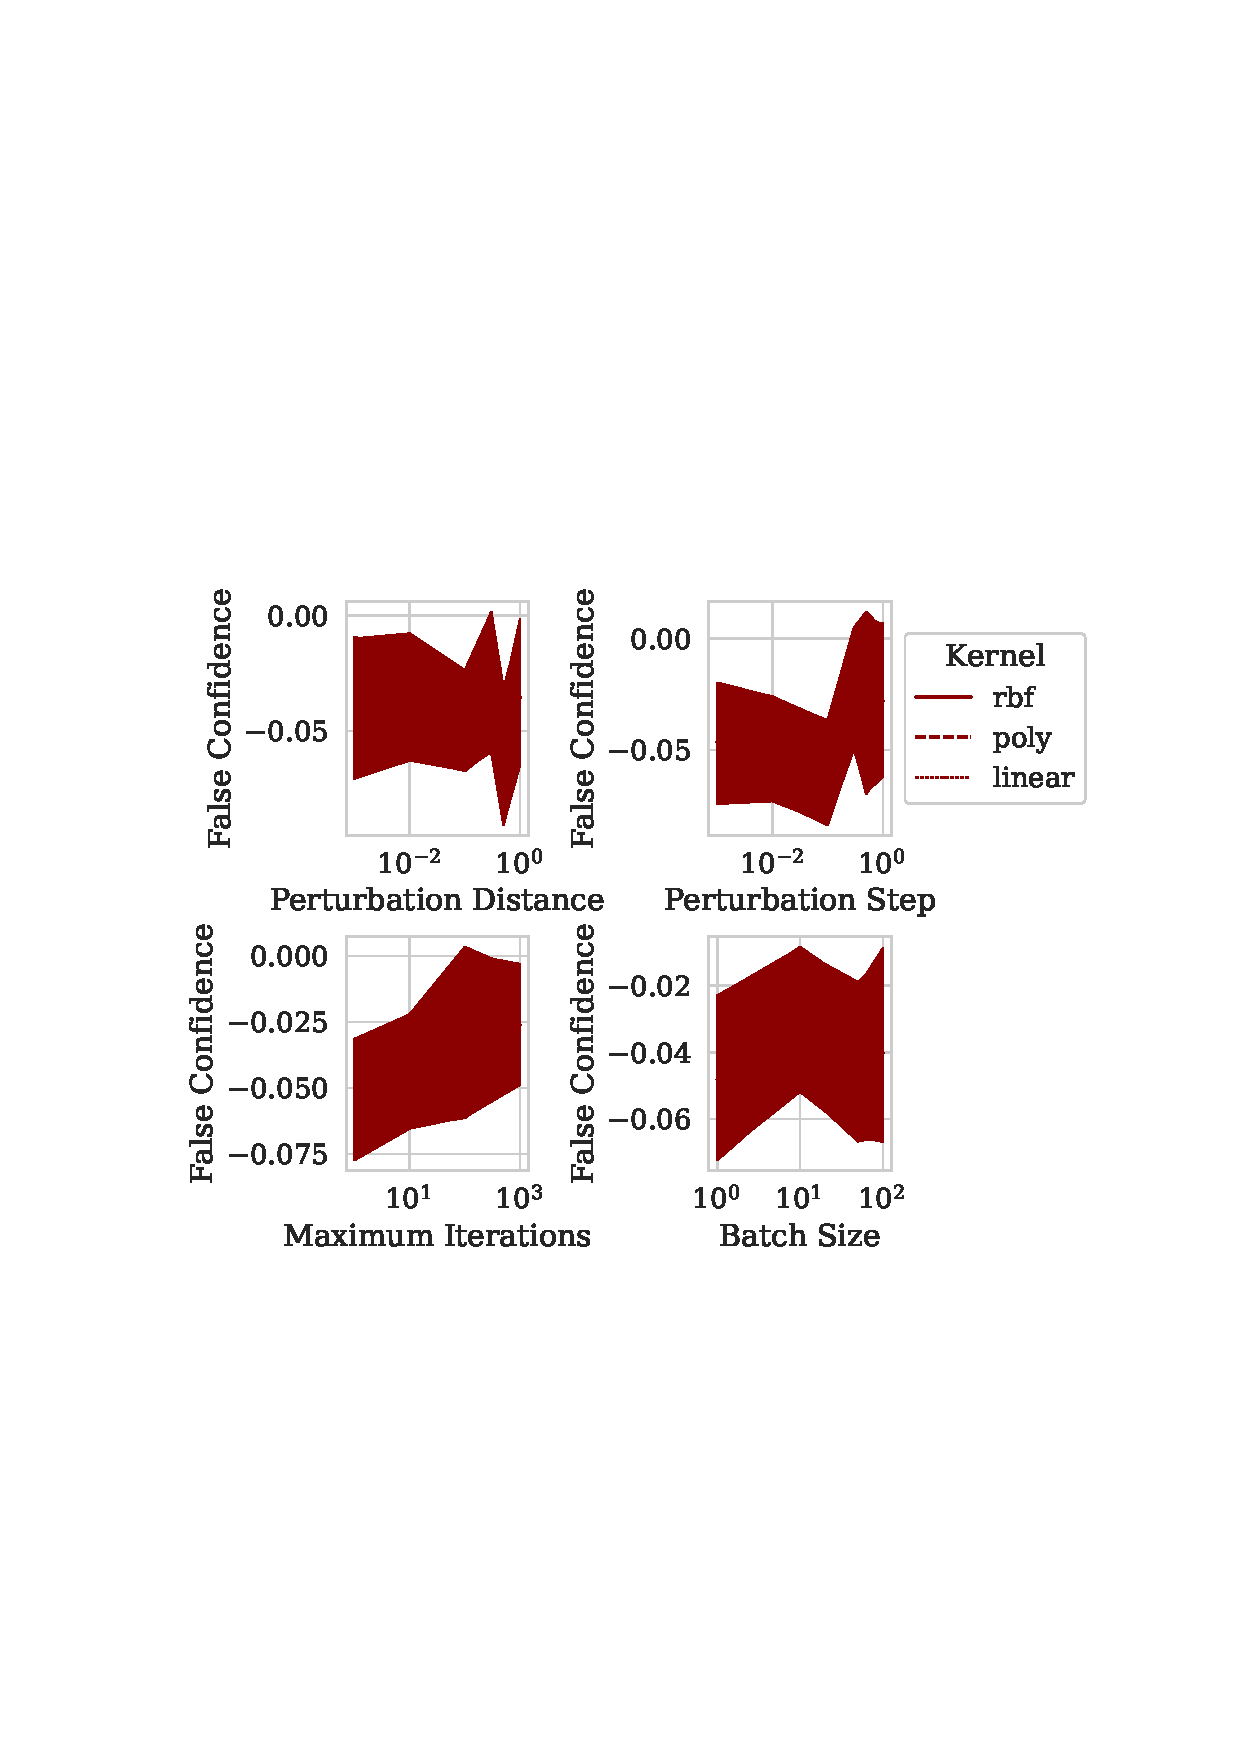
\includegraphics[width=\textwidth]{./kdd-nsl/retrain_confidence_vs_attack_parameters.pdf}
     \end{subfigure}
     \hfill
     \caption{Efficacy of Adversarial Retraining on KDD-NSL Dataset. The top left depicts the adversarial and benign accuracy over a number of retraining epochs. The top right depicts the per epoch training time as the number of training epochs increases. The bottom row depicts the false confidence before retraining (left) on strong adversarial examples and after (right).}
     \label{fig:kdd-nsl}
\end{figure*}
